\documentclass{beamer}

% TODO: print out https://www.fuzzingbook.org/code/Intro_Testing.py

\usetheme{Boadilla}

%\includeonlyframes{current}

\usepackage{times}
\usefonttheme{structurebold}
\usepackage{listings}

\usepackage{pgf}
\usepackage{tikz}
\usepackage{alltt}
\usepackage[normalem]{ulem}
\usetikzlibrary{arrows}
\usetikzlibrary{automata}
\usetikzlibrary{shapes}
\usepackage{amsmath,amssymb}
\usepackage{rotating}
\usepackage{ulem}
\usepackage{pythonhighlight}

\usetikzlibrary{arrows,automata,shapes}
\tikzstyle{block} = [rectangle, draw, fill=blue!20, 
    text width=5em, text centered, rounded corners, minimum height=2em]
\tikzstyle{bt} = [rectangle, draw, fill=blue!20, 
    text width=4em, text centered, rounded corners, minimum height=2em]

\lstdefinelanguage{JavaScript}{
  keywords={typeof, new, true, false, catch, function, return, null, catch, switch, var, if, in, while, 
do, else, case, break},
  keywordstyle=\color{blue}\bfseries,
  ndkeywords={class, export, boolean, throw, implements, import, this},
  ndkeywordstyle=\color{darkgray}\bfseries,
  identifierstyle=\color{black},
  sensitive=false,
  comment=[l]{//},
  morecomment=[s]{/*}{*/},
  commentstyle=\color{purple}\ttfamily,
  stringstyle=\color{red}\ttfamily,
  morestring=[b]',
  morestring=[b]''
}

%\setbeamercovered{dynamic}
\setbeamertemplate{footline}[page number]{}
\setbeamertemplate{navigation symbols}{}
\usefonttheme{structurebold}

\title{Software Testing, Quality Assurance \& Maintenance---Lecture 8}
\author{Patrick Lam\\University of Waterloo}
\date{January 30, 2026}

\colorlet{redshaded}{red!25!bg}
\colorlet{shaded}{black!25!bg}
\colorlet{shadedshaded}{black!10!bg}
\colorlet{blackshaded}{black!40!bg}

\colorlet{darkred}{red!80!black}
\colorlet{darkblue}{blue!80!black}
\colorlet{darkgreen}{green!80!black}

\newcommand{\rot}[1]{\rotatebox{90}{\mbox{#1}}}
\newcommand{\gray}[1]{\mbox{#1}}

\newenvironment{changemargin}[1]{% 
  \begin{list}{}{% 
    \setlength{\topsep}{0pt}% 
    \setlength{\leftmargin}{#1}% 
    \setlength{\rightmargin}{1em}
    \setlength{\listparindent}{\parindent}% 
    \setlength{\itemindent}{\parindent}% 
    \setlength{\parsep}{\parskip}% 
  }% 
  \item[]}{\end{list}}



\begin{document}

\usebackgroundtemplate{\tikz\node[opacity=0.1]{\includegraphics[width=\paperwidth]{L02/07172_about_banmochi_ishi_strength_and_grip_testing.JPG}};}
\begin{frame}
  \titlepage
\end{frame}

\usebackgroundtemplate{\tikz\node[opacity=0.3]{\includegraphics[width=\paperwidth]{L04/20241110_001424746_blackbird.jpg}};}
\part{Mutation-Based Fuzzing}
\begin{frame}
  \partpage
\end{frame}
\usebackgroundtemplate{}

\begin{frame}
  \frametitle{Putting things together}

  \Large
  \begin{changemargin}{2em}
    Goal: generate many test cases automatically.\\[1em]
    When we talked about helping human oracles,\\
    we mentioned starting from known inputs.\\[1em]
    \alert{Mutation-based fuzzing}: automatically modify known inputs.
  \end{changemargin}
\end{frame}

\begin{frame}
  \frametitle{Mutation-based fuzzing in practice}

  \Large
  \begin{changemargin}{2em}
    Could just flip bytes in the input.\\[1em]

    Or, parse the input and change some nonterminals in the AST.\\[1em]

    Note: Also need to update checksums to see anything interesting.
  \end{changemargin}
\end{frame}

\begin{frame}[fragile]
  \frametitle{Example: URLs}

  \Large
  \begin{changemargin}{2em}
A valid URL looks like this:
\begin{center}
  \small
\begin{verbatim}
    scheme://netloc/path?query#fragment
\end{verbatim}
\end{center}

There is a definition of valid vs invalid URLs (RFC 3986).\\[1em]

A program should do something useful with valid URLs and reject invalid URLs.\\[1em]
Let's use fuzzing to generate valid and invalid URLs.

  \end{changemargin}
\end{frame}

\begin{frame}[fragile]
  \frametitle{schemes}

  \Large
  \begin{changemargin}{2em}
\begin{center}
  \small
\begin{verbatim}
    scheme://netloc/path?query#fragment
\end{verbatim}
\end{center}
~\\[1em]
There are a fixed number of valid \texttt{scheme}s:
\texttt{http}, \texttt{https}, \texttt{file}, etc.

  \end{changemargin}
\end{frame}

\begin{frame}[fragile]
  \frametitle{Using the urllib library}

  \small
  \begin{changemargin}{2em}
\begin{lstlisting}[language=Python]
>>> from typing import Tuple, List
>>> from typing import Callable, Set, Any
>>> from urllib.parse import urlparse

>>> urlparse("http://www.google.com/search?q=fuzzing")
ParseResult(scheme='http', netloc='www.google.com',
  path='/search', params='',
  query='q=fuzzing', fragment='')
\end{lstlisting}
  \end{changemargin}
\end{frame}

\begin{frame}[fragile]
  \frametitle{urllib in ur function}

  \Large
  \begin{changemargin}{2em}
    \begin{python}
def url_consumer(url: str) -> bool:
    supported_schemes = ["http", "https"]
    result = urlparse(url)
    if result.scheme not in supported_schemes:
        raise ValueError("Scheme must be one of " + 
                         repr(supported_schemes))
    if result.netloc == '':
        raise ValueError("Host must be non-empty")

    # Do something with the URL
    return True
    \end{python}
    How to test?
  \end{changemargin}
\end{frame}

\begin{frame}[fragile]
  \frametitle{Naive input generation}

  \Large
  \begin{changemargin}{2em}
  In \texttt{code/L08/random\_inputs.py}:
\begin{python}
  for i in range(1000):
    try:
        fuzzer = Fuzzer()
        url = fuzzer.fuzzer()
        result = url_consumer(url)
        print("Success!")
    except ValueError:
        pass
\end{python}
You'd be very lucky indeed to see Success!.\\[1em]
Basically, this fuzzing won't test anything past validation.
  \end{changemargin}
\end{frame}

\begin{frame}[fragile]
  \frametitle{Being less naive}

  \Large
  \begin{changemargin}{2em}
    Basically two alternatives:
    \begin{itemize}
    \item mutate existing inputs; or,
    \item generate inputs using a grammar.
    \end{itemize}
    ~\\[1em]
    (As mentioned earlier, can also parse/mutate/unparse).
  \end{changemargin}
\end{frame}

\begin{frame}[fragile]
  \frametitle{Mutating existing inputs (strings)}
  \begin{python}
import random

def delete_random_character(s: str) -> str:
    """Returns s with a random character deleted"""
    if s == "":
        return s

    pos = random.randint(0, len(s) - 1)
    #print("Deleting", repr(s[pos]), "at", pos)
    return s[:pos] + s[pos + 1:]

def insert_random_character(s: str) -> str:
    """Returns s with a random character inserted"""
    pos = random.randint(0, len(s))
    random_character = chr(random.randrange(32, 127))
    #print("Inserting", repr(random_character), "at", pos)
    return s[:pos] + random_character + s[pos:]
  \end{python}
\end{frame}

\begin{frame}[fragile]
  \frametitle{Mutating existing inputs (strings)}
  \begin{python}
def flip_random_character(s):
    """Returns s with a random bit flipped in a random position"""
    if s == "":
        return s

    pos = random.randint(0, len(s) - 1)
    c = s[pos]
    bit = 1 << random.randint(0, 6)
    new_c = chr(ord(c) ^ bit)
    #print("Flipping", bit, "in", repr(c) + ", giving", repr(new_c))
    return s[:pos] + new_c + s[pos + 1:]
  \end{python}
\end{frame}

\begin{frame}[fragile]
  \frametitle{Running the mutation code}
  \begin{python}
seed_input = "A quick brown fox"
for i in range(10):
    x = delete_random_character(seed_input)
    print(repr(x))

for i in range(10):
    print(repr(insert_random_character(seed_input)))

for i in range(10):
    print(repr(flip_random_character(seed_input)))
  \end{python}
\end{frame}


\begin{frame}[fragile]
  \frametitle{Choose randomness randomly}
  \begin{python}
def mutate(s: str) -> str:
    """Return s with a random mutation applied"""
    mutators = [
        delete_random_character,
        insert_random_character,
        flip_random_character
    ]
    mutator = random.choice(mutators)
    # print(mutator)
    return mutator(s)

for i in range(10):
    print(repr(mutate("A quick brown fox")))
  \end{python}
\end{frame}

\begin{frame}[fragile]
  \frametitle{Back to URLs: retrofitting \texttt{url\_consumer}}
  \begin{python}
from random_inputs import url_consumer

def is_valid_url(url: str) -> bool:
    try:
        result = url_consumer(url)
        return True
    except ValueError:
        return False

assert is_valid_url("http://www.google.com/search?q=fuzzing")
assert not is_valid_url("xyzzy")
  \end{python}
  Easier to test with this wrapper.
\end{frame}

\begin{frame}[fragile]
  \frametitle{Using the mutation fuzzer}
  \begin{python}
from mutation_fuzzer import MutationFuzzer

seed_input = "http://www.google.com/search?q=fuzzing"
valid_inputs = set()
trials = 20

mutation_fuzzer = MutationFuzzer([])
for i in range(trials):
    inp = mutation_fuzzer.mutate(seed_input)
    if is_valid_url(inp):
        valid_inputs.add(inp)

print (len(valid_inputs)/trials)
  \end{python}
  What do you observe when you run this?
\end{frame}

\begin{frame}
  \frametitle{Exercise: \texttt{http} $\rightarrow$ \texttt{https}}

  \Large
  \begin{changemargin}{2em}
    How long should you expect to wait before randomly mutating \texttt{http} to \texttt{https}
    and getting a valid input?
  \end{changemargin}
\end{frame}

\begin{frame}[fragile]
  \frametitle{Multiple mutations}

  \Large
  \begin{changemargin}{2em}
  Not for mutation analysis, but useful here.

\begin{python}
seed_input = "http://www.google.com/search?q=fuzzing"
mutations = 50
inp = seed_input
for i in range(mutations):
    if i % 5 == 0:
        print(i, "mutations:", repr(inp))
    inp = mutation_fuzzer.mutate(inp)
\end{python}
  \end{changemargin}
\end{frame}

\begin{frame}[fragile]
  \frametitle{Encapsulating fuzzing in a class}

  \Large
  \begin{changemargin}{2em}
\begin{python}
class MutationFuzzer(Fuzzer):
    """Base class for mutational fuzzing"""

    def __init__(self, seed: List[str],
                 min_mutations: int = 2,
                 max_mutations: int = 10) -> None
        # ...
    def reset(self) -> None:
        # ...
\end{python}

  \end{changemargin}
\end{frame}

\begin{frame}[fragile]
  \frametitle{Useful functions}

  \Large
  \begin{changemargin}{2em}
\begin{python}
    def create_candidate(self) -> str:
        """Create a new candidate by mutating a population member"""
        candidate = random.choice(self.population)
        trials = random.randint(self.min_mutations, self.max_mutations)
        for i in range(trials):
            candidate = self.mutate(candidate)
        return candidate

    def fuzz(self) -> str:
        if self.seed_index < len(self.seed):
            # Still seeding
            self.inp = self.seed[self.seed_index]
            self.seed_index += 1
        else:
            # Mutating
            self.inp = self.create_candidate()
        return self.inp
\end{python}

  \end{changemargin}
\end{frame}

\begin{frame}[fragile]
  \frametitle{Using MutationFuzzer}

  \Large
  \begin{changemargin}{0em}
\begin{python}
>>> seed_input = "http://www.google.com/search?q=fuzzing"
>>> mutation_fuzzer = MutationFuzzer(seed=[seed_input])
>>> print(mutation_fuzzer.fuzz())
>>> print(mutation_fuzzer.fuzz())
>>> print(mutation_fuzzer.fuzz())
http://www.google.com/search?q=fuzzing
http+:R/'ww.google.com/serchql=fuzing
htEtp://wwwgoogld.coi/earch?qn=fung
\end{python}
  \end{changemargin}
\end{frame}

\part{Intermission: Guiding by Coverage}
\begin{frame}
  \partpage
\end{frame}

\usebackgroundtemplate{\tikz\node[opacity=0.3]{\includegraphics[width=\paperwidth]{L08/6367_step_pyramid_with_scaffolding.jpg}};}
\begin{frame}
  \frametitle{On Hierarchies}

    \Large
  \begin{changemargin}{2em}
    We know that randomly changing bytes won't exercise much interesting functionality.\\[1em]
    It can cause crashes, though, at least for a while.\\[1em]
    Let's continue to use randomness, but in a more directed way.
  \end{changemargin}
\end{frame}


\begin{frame}
  \frametitle{Hierarchy of inputs: C}
  \begin{changemargin}{1em}
    C programs are way more structured than URLs.
\begin{enumerate}
\item sequence of ASCII characters;
\item sequence of words, separators, and white space (gets past the lexer);
\item syntactically correct C program (gets past the parser);
\item type-correct C program (gets past the type checker);
\item statically conforming C program (starts to exercise optimizations);
\item dynamically conforming C program;
\item model conforming C program.
\end{enumerate}
~\\[1em]
Each level is a subset of previous level, but more likely to find interesting inputs specific to the system.\\[1em]
Operate at all the levels.
  \end{changemargin}
\end{frame}

\begin{frame}
  \frametitle{Generating higher-level inputs}

  \Large
  \begin{changemargin}{2em}
    Two choices:
    \begin{enumerate}
    \item use grammars (context-free grammars still don't satisfy all constraints)
    \item modify existing inputs (as seen above)
    \end{enumerate}

    ~\\[1em]
    This is true for all generational fuzzing tools. \\
    Need to incorporate knowledge about correct syntax.
  \end{changemargin}
\end{frame}
\usebackgroundtemplate{}

\part{Guiding by Coverage}
\begin{frame}
  \partpage
\end{frame}

\usebackgroundtemplate{\tikz\node[opacity=0.3]{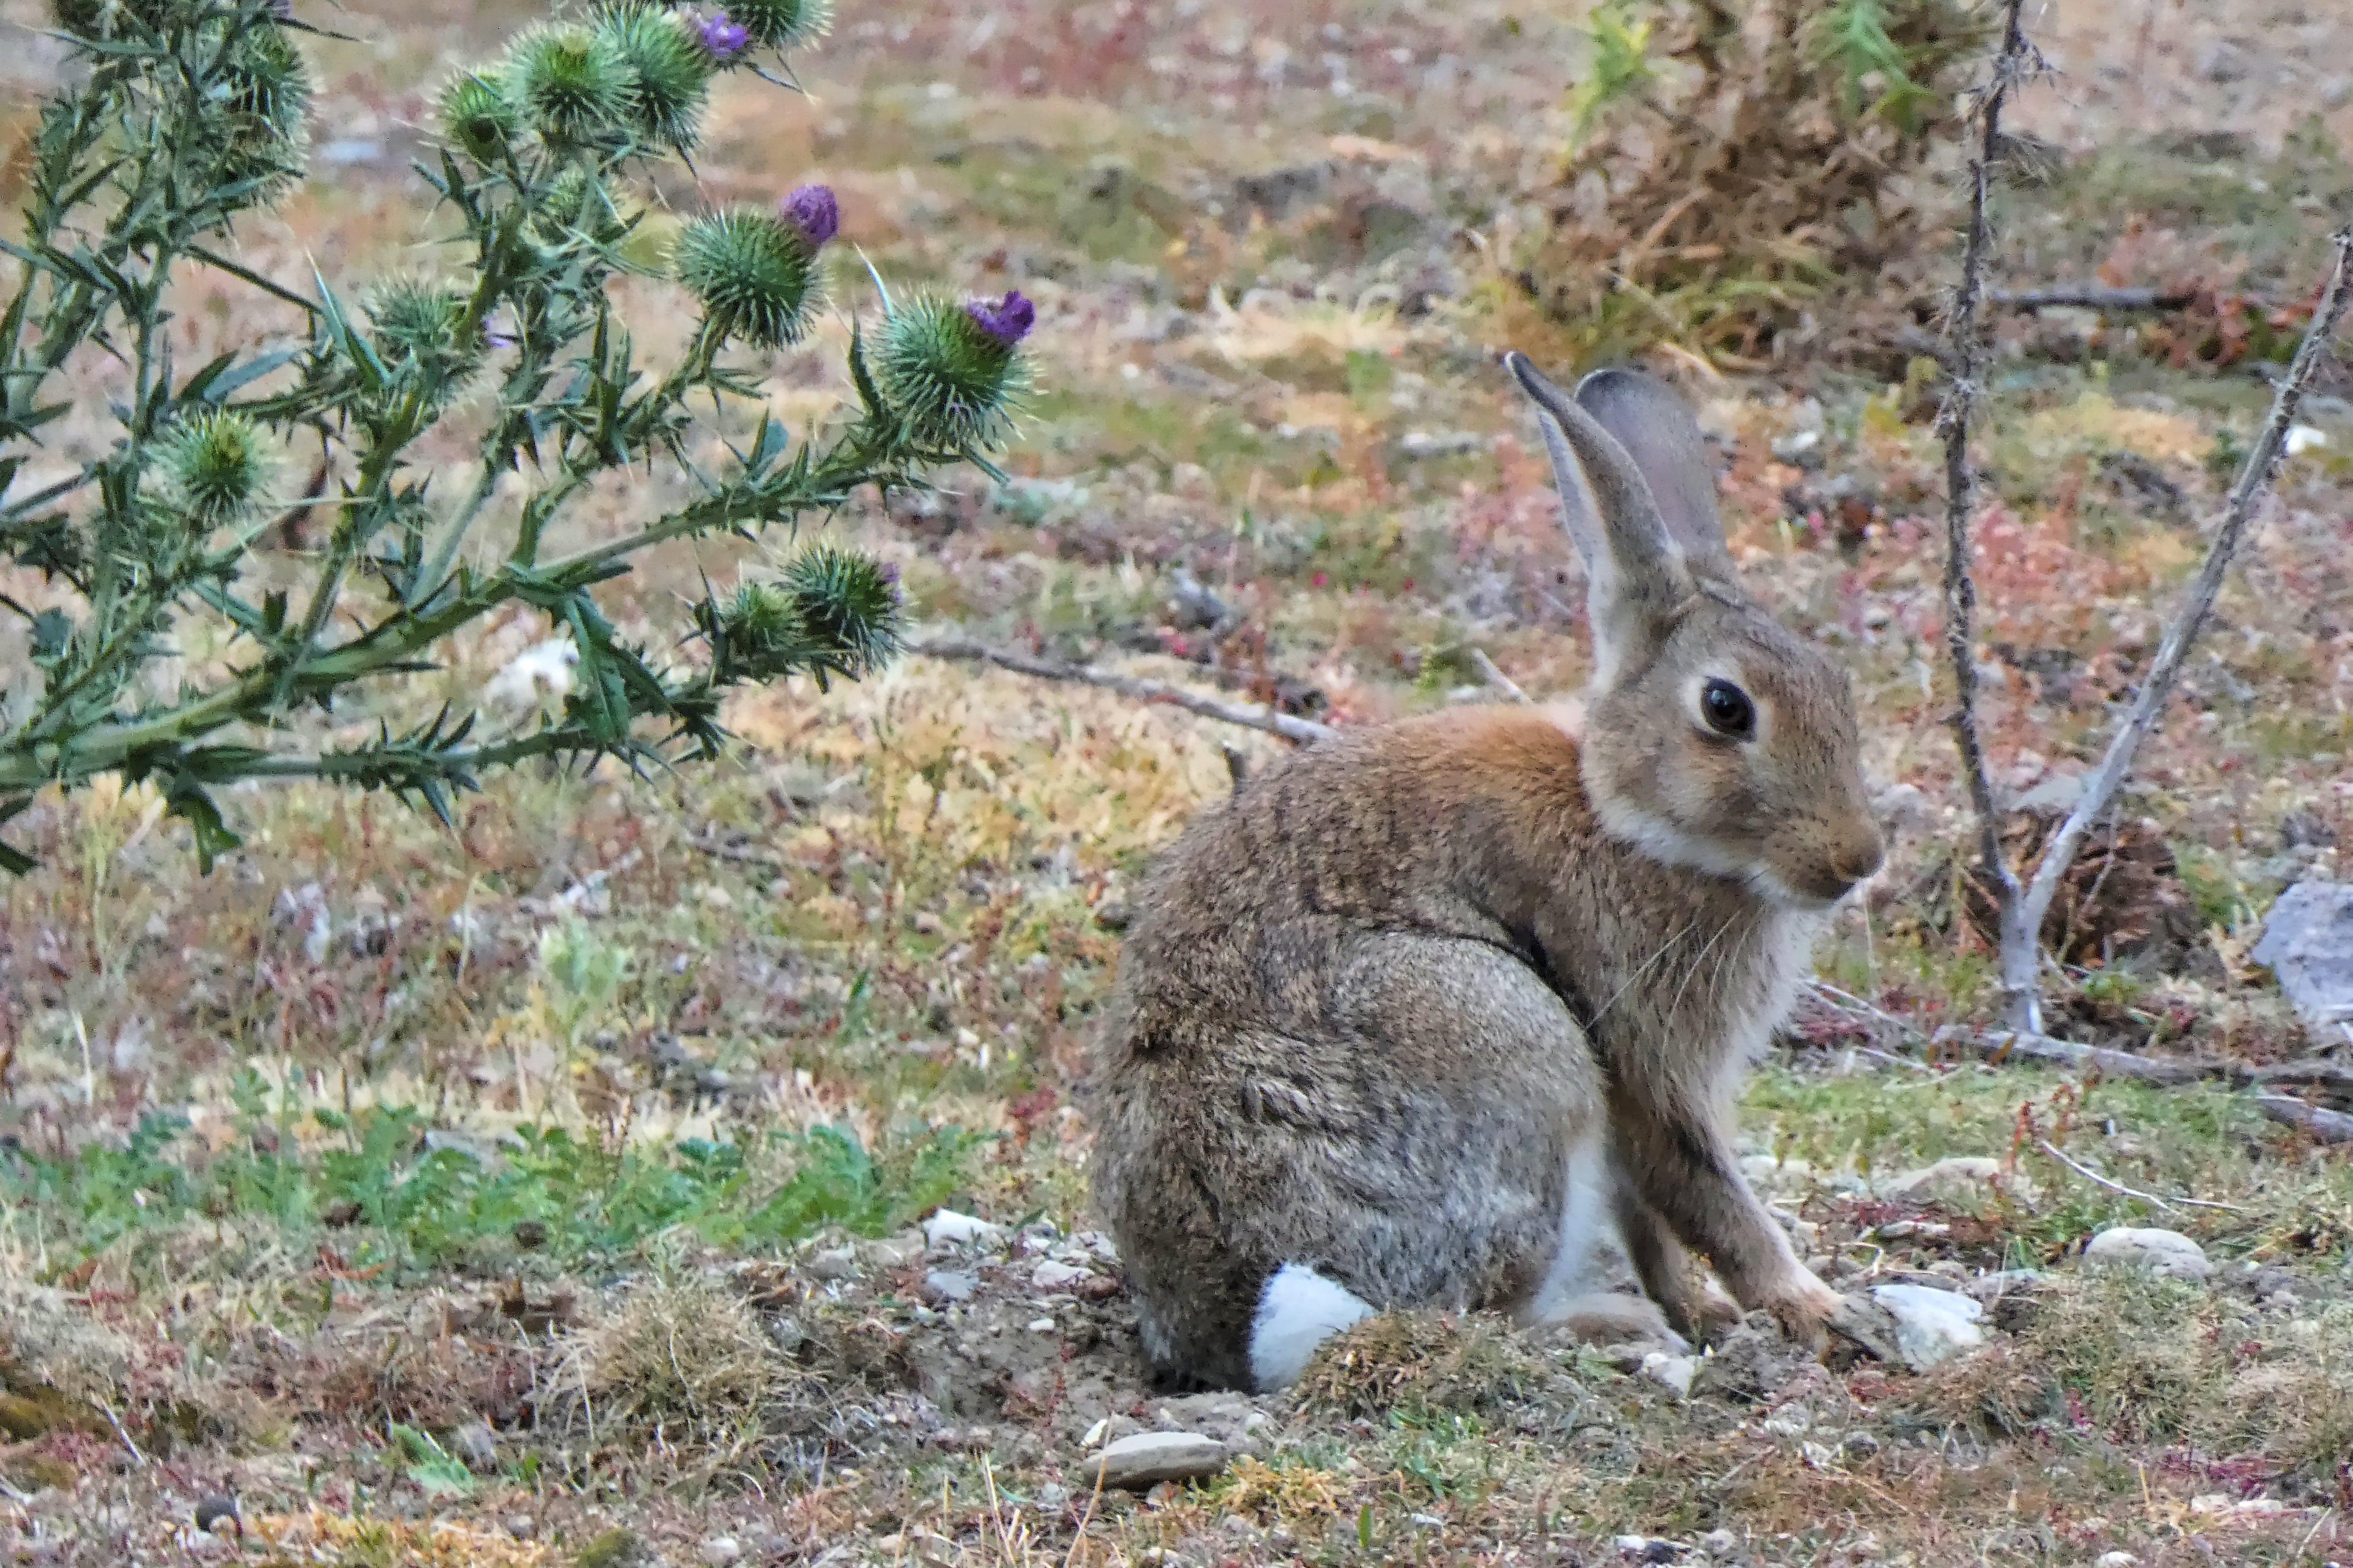
\includegraphics[width=\paperwidth]{L08/00296_bunny_v1.jpg}};}
\begin{frame}
  \frametitle{AFL's big idea}

  \Large
  \begin{changemargin}{2em}
    So far: use coverage to evaluate test suites.\\[1em]
    New: use coverage to guide test generation (AFL).
  \end{changemargin}
\end{frame}
\usebackgroundtemplate{}

\begin{frame}[fragile]
  \frametitle{Infrastructure}
  \begin{changemargin}{2em}
\begin{python}
class Runner:
    """Base class for testing inputs."""

    # Test outcomes
    PASS = "PASS"
    FAIL = "FAIL"
    UNRESOLVED = "UNRESOLVED"

    def __init__(self) -> None:
        """Initialize"""
        pass

    def run(self, inp: str) -> Any:
        """Run the runner with the given input"""
        return (inp, Runner.UNRESOLVED)
\end{python}
  \end{changemargin}
\end{frame}

\begin{frame}[fragile]
  \frametitle{Instantiating infrastructure}
  \begin{changemargin}{2em}
\begin{python}
class FunctionRunner(Runner):
    def __init__(self, function: Callable) -> None:
        self.function = function

    def run_function(self, inp: str) -> Any:
        return self.function(inp)

    def run(self, inp: str) -> Tuple[Any, str]:
        try:
            result = self.run_function(inp)
            outcome = self.PASS
        except Exception:
            result = None
            outcome = self.FAIL
        return result, outcome
\end{python}
  \end{changemargin}
\end{frame}

\begin{frame}[fragile]
  \frametitle{Running the FunctionRunner}
  \begin{changemargin}{2em}
\begin{python}
from fuzzer import Runner
from random_inputs import url_consumer
from urllib.parse import urlparse
    
if __name__ == "__main__":
    # view output from urlconsumer_runner:
    urlconsumer_runner = FunctionRunner(url_consumer)
    print (urlconsumer_runner.run("https://foo.bar"))
\end{python}

Output: \texttt{(True, 'PASS')}
  \end{changemargin}
\end{frame}

\begin{frame}[fragile]
  \frametitle{Measuring Coverage in the Runner}
  \begin{changemargin}{2em}
\begin{python}
class FunctionCoverageRunner(FunctionRunner):
    def run_function(self, inp: str) -> Any:
        with Coverage() as cov:
            try:
                result = super().run_function(inp)
            except Exception as exc:
                self._coverage = cov.coverage()
                raise exc

        self._coverage = cov.coverage()
        return result

    def coverage(self) -> Set[Location]:
        return self._coverage
\end{python}
  \end{changemargin}
\end{frame}

\begin{frame}[fragile]
  \frametitle{Running \texttt{function\_coverage\_runner.py}}
  \begin{changemargin}{2em}
\begin{python}
if __name__ == "__main__":
    from urllib.parse import urlparse

    # view output from urlconsumer_runner:
    urlconsumer_runner = FunctionCoverageRunner(url_consumer)
    urlconsumer_runner.run("https://foo.bar")

    print(list(urlconsumer_runner.coverage())[:5])
\end{python}
prints a slice of the coverage:
{\small \begin{verbatim}
  [('url_consumer', 7), ('_splitnetloc', 416),
    ('_splitnetloc', 419), ('urlsplit', 502),
    ('urlsplit', 499)]
\end{verbatim} }
  \end{changemargin}
\end{frame}

\begin{frame}
  \frametitle{Putting the AFL Idea into Practice}

  \Large
  \begin{changemargin}{2em}
    Maintain a population of source inputs.\\[1em]
    Add an input to the population when the input adds to coverage.\\[1em]
    The mutation fuzzer (from Part I) mutates inputs in the population to generate new candidate inputs.
  \end{changemargin}
\end{frame}

\begin{frame}[fragile]
  \frametitle{{\texttt MutationCoverageFuzzer} implementation}
\begin{python}
class MutationCoverageFuzzer(MutationFuzzer):
    def reset(self) -> None:
        super().reset()
        self.coverages_seen: Set[frozenset] = set()
        self.population = []

    def run(self, runner: FunctionCoverageRunner) -> Any:
        """Run function(inp) while tracking coverage.
           If we reach new coverage,
           add inp to population and its coverage to population_coverage
        """
        result, outcome = super().run(runner)
        new_coverage = frozenset(runner.coverage())
        if outcome == Runner.PASS and new_coverage not in self.coverages_seen:
            # We have new coverage
            self.population.append(self.inp)
            self.coverages_seen.add(new_coverage)

        return result
\end{python}
\end{frame}

\begin{frame}[fragile]
  \frametitle{The population}
  \begin{python}
if __name__ == "__main__":
    seed_input = "http://www.google.com/search?q=fuzzing"
    mutation_fuzzer = MutationCoverageFuzzer(seed=[seed_input])
    urlconsumer_runner = FunctionCoverageRunner(url_consumer)
    mutation_fuzzer.runs(urlconsumer_runner, trials=10000)
    print (mutation_fuzzer.population)
  \end{python}
  We aim to increase coverage of \texttt{url\_consumer} and functions it calls.
  The population after 10,000 trials:
  {\scriptsize
    \begin{verbatim}
      ['http://www.google.com/search?q=fuzzing',
        'http://www.google|.com/search\x7fq=fuZzing',
        'http://ww;w.google|.com/searc\x7f=fuZzing#',
        'http://ww;w?.gogle|com/sEarc\x7f=f,uZzig#',
        "http://www.googla|.com'sarch\x7fq9fuZzi!ng",
        'http://ww;wgoole|/com/sear;c\x7ffuZzing#',
        'http://wg;wgoole|m/cnmb/suar;cwfuZzing\x03',
        'http://wg;wgoole|m/cnmb/suar;cwfuZzing\x03',
        'http://wgW;wgoole|m/cnmb/s}ar;cwfuZz-ing\x03/:',
        'http://wgW;wgoole|m/cnmb/s}ar;cwfuZz?-qing\x03/:',
        'Http://wg5W;\x7fgoorle|amcmb/S}ar;cwfuZz?-qing#\x03/:',
        'Http://wg5W;\x7fgoOrle|!mcmb/S}ap;cwfuZj/-qing#/:']
\end{verbatim}
    }

\end{frame}

\begin{frame}
  \frametitle{Coverage-guided fuzzing summary}

  \Large
  \begin{changemargin}{2em}
    It is possible to plot coverage-over-time using this strategy;
    see the \emph{Fuzzing Book} for details.\\[1em]
    Coverage-guided fuzzing (AFL) definitely explores new parts of the program's
    behaviour as it runs.\\[1em]
    Eventually, it hits diminishing returns.
  \end{changemargin}
\end{frame}


\end{document}
